% !TEX program = pdflatex
\documentclass[a4paper,14pt]{extarticle}

% ===== Язык и кодировка =====
\usepackage[T2A]{fontenc}
\usepackage[utf8]{inputenc}
\usepackage[russian,english]{babel}

% ===== Поля =====
\usepackage[left=30mm, right=15mm, top=20mm, bottom=20mm]{geometry}

% ===== Графика и таблицы =====
\usepackage{graphicx}
\usepackage{longtable}
\usepackage{array}
\usepackage{booktabs}
\usepackage{tabularx}
\usepackage{float}
\usepackage{pdflscape}

% ===== Листинги кода =====
\usepackage{listings}
\usepackage{etoolbox}

\lstset{
  inputencoding=utf8,
  extendedchars=true,
  keepspaces=true,
  literate=
   {а}{{\selectfont\char224}}1 {б}{{\selectfont\char225}}1
   {в}{{\selectfont\char226}}1 {г}{{\selectfont\char227}}1
   {д}{{\selectfont\char228}}1 {е}{{\selectfont\char229}}1
   {ё}{{\"e}}1
   {ж}{{\selectfont\char230}}1 {з}{{\selectfont\char231}}1
   {и}{{\selectfont\char232}}1 {й}{{\selectfont\char233}}1
   {к}{{\selectfont\char234}}1 {л}{{\selectfont\char235}}1
   {м}{{\selectfont\char236}}1 {н}{{\selectfont\char237}}1
   {о}{{\selectfont\char238}}1 {п}{{\selectfont\char239}}1
   {р}{{\selectfont\char240}}1 {с}{{\selectfont\char241}}1
   {т}{{\selectfont\char242}}1 {у}{{\selectfont\char243}}1
   {ф}{{\selectfont\char244}}1 {х}{{\selectfont\char245}}1
   {ц}{{\selectfont\char246}}1 {ч}{{\selectfont\char247}}1
   {ш}{{\selectfont\char248}}1 {щ}{{\selectfont\char249}}1
   {ъ}{{\selectfont\char250}}1 {ы}{{\selectfont\char251}}1
   {ь}{{\selectfont\char252}}1 {э}{{\selectfont\char253}}1
   {ю}{{\selectfont\char254}}1 {я}{{\selectfont\char255}}1
   {А}{{\selectfont\char192}}1 {Б}{{\selectfont\char193}}1
   {В}{{\selectfont\char194}}1 {Г}{{\selectfont\char195}}1
   {Д}{{\selectfont\char196}}1 {Е}{{\selectfont\char197}}1
   {Ё}{{\"E}}1
   {Ж}{{\selectfont\char198}}1 {З}{{\selectfont\char199}}1
   {И}{{\selectfont\char200}}1 {Й}{{\selectfont\char201}}1
   {К}{{\selectfont\char202}}1 {Л}{{\selectfont\char203}}1
   {М}{{\selectfont\char204}}1 {Н}{{\selectfont\char205}}1
   {О}{{\selectfont\char206}}1 {П}{{\selectfont\char207}}1
   {Р}{{\selectfont\char208}}1 {С}{{\selectfont\char209}}1
   {Т}{{\selectfont\char210}}1 {У}{{\selectfont\char211}}1
   {Ф}{{\selectfont\char212}}1 {Х}{{\selectfont\char213}}1
   {Ц}{{\selectfont\char214}}1 {Ч}{{\selectfont\char215}}1
   {Ш}{{\selectfont\char216}}1 {Щ}{{\selectfont\char217}}1
   {Ъ}{{\selectfont\char218}}1 {Ы}{{\selectfont\char219}}1
   {Ь}{{\selectfont\char220}}1 {Э}{{\selectfont\char221}}1
   {Ю}{{\selectfont\char222}}1 {Я}{{\selectfont\char223}}1
}

\usepackage{xcolor}
\usepackage{fancyvrb}

\colorlet{lststringcolor}{red!70!black}

\lstset{
  language=C,
  basicstyle=\footnotesize\ttfamily,
  keywordstyle=\color{blue}\bfseries,
  commentstyle=\color{gray}\itshape,
  stringstyle=\color{lststringcolor},
  numbers=left,
  numberstyle=\tiny\color{gray},
  numbersep=8pt,
  frame=single,
  breaklines=true,
  breakatwhitespace=false,
  columns=fullflexible,
  tabsize=4,
  showstringspaces=false,
  captionpos=b,
  postbreak=\mbox{$\hookrightarrow$\space},
}

% ===== Блок сложности =====
\newcommand{\opcount}[2]{%
  \par\vspace{2pt}%
  \noindent
  \colorbox{gray!15}{%
    \parbox{\dimexpr\linewidth-2\fboxsep\relax}{%
      \small\bfseries\ttfamily\raggedright #1:\enskip #2%
    }%
  }%
  \par\vspace{6pt}%
}

% ===== Гиперссылки =====
\PassOptionsToPackage{hyphens}{url}
\usepackage{amsmath}
\usepackage{hyperref}
\hypersetup{
  colorlinks=true,
  linkcolor=black,
  urlcolor=blue,
  citecolor=black,
}

% ===== Отступ первого абзаца =====
\usepackage{indentfirst}
\setlength{\parindent}{1.25cm}

% ===== Межстрочный интервал =====
\usepackage{setspace}
\onehalfspacing

% ===== Заголовки разделов =====
\usepackage{titlesec}
\titleformat{\section}{\normalfont\large\bfseries\centering}{\thesection.}{0.5em}{}
\titleformat{\subsection}{\normalfont\normalsize\bfseries}{\thesubsection.}{0.5em}{}

% ===== Перенос слов =====
\usepackage{ragged2e}
\emergencystretch=6em
\tolerance=9999
\hbadness=10001

\DeclareUrlCommand\code{\urlstyle{tt}}
\newcommand{\tcode}[1]{\code{#1}}

% ===== Подписи рисунков =====
\usepackage{caption}
\captionsetup{justification=centering, labelsep=endash}

\begin{document}

% ===================== ТИТУЛЬНЫЙ ЛИСТ =====================
\begin{titlepage}
\begin{center}

\textbf{Национальный исследовательский университет ИТМО}\\[0.5cm]
\textbf{Факультет безопасности информационных технологий}\\[1cm]

{\Large\textbf{Алгоритмы и структуры данных}}\\[1cm]
{\large Лабораторная работа №4}\\[0.5cm]
{\large\textbf{<<Цифровая сортировка стека на базе массива с поиском методом Бойера-Мура и записью результата в красно-чёрное дерево>>}}\\[3cm]

\begin{flushright}
\begin{minipage}{0.35\textwidth}
\textbf{Выполнил:}\\
Студент группы N3247\\
Сивоконь А.А.\\[1cm]

\noindent\rule{5cm}{0.4pt}\\
\centerline{(подпись)}

\vspace{0.5cm}

\textbf{Преподаватель:}\\
Ерофеев С.А.\\[1cm]
\noindent\rule{5cm}{0.4pt}\\
\centerline{(отметка о выполнении)}

\vspace{1.5cm}

\noindent\rule{5cm}{0.4pt}\\
\centerline{(подпись)}
\end{minipage}
\end{flushright}

\vfill

Санкт-Петербург\\
2026

\end{center}
\end{titlepage}

% ===================== СОДЕРЖАНИЕ =====================
\newpage
\renewcommand{\contentsname}{Содержание}
\tableofcontents

% ===================== 1. ПОСТАНОВКА ЗАДАЧИ =====================
\newpage
\section{Постановка задачи}

\textbf{Цель работы:} разработать программу цифровой сортировки (Radix Sort LSD) для последовательности целых чисел (включая отрицательные), считываемых из файла, используя в качестве основной и вспомогательной структуры данных \textbf{стек на базе динамического массива}; реализовать \textbf{поиск методом Бойера-Мура} в отсортированном стеке; записать результат сортировки в \textbf{красно-чёрное дерево}; определить сложность программы.

\vspace{0.5cm}
\textbf{Для достижения поставленной цели необходимо решить следующие задачи:}
\begin{enumerate}
  \item Реализовать стек на динамическом массиве с операциями \texttt{stack\_init}, \texttt{stack\_push}, \texttt{stack\_pop}, \texttt{stack\_peek}, \texttt{stack\_is\_empty}, \texttt{stack\_free} (с автоматическим расширением);
  \item Реализовать алгоритм цифровой сортировки LSD через 10 стеков-корзин с учётом LIFO-особенностей (дополнительные реверсы для устойчивости);
  \item Корректно обработать отрицательные числа: разделить стек на два вспомогательных, отсортировать каждый независимо, объединить результат с правильным порядком;
  \item Реализовать поиск методом Бойера-Мура: сериализация отсортированного стека в строку с разделителями, поиск целыми токенами, возврат позиции числа (а не символа);
  \item Реализовать красно-чёрное дерево и записать в него результат сортировки (с выводом inorder-обхода для проверки);
  \item Оценить теоретическую сложность алгоритмов;
  \item Провести тестирование программы на различных наборах данных;
  \item Составить блок-схемы алгоритма и оформить отчёт.
\end{enumerate}

% ===================== 2. ОПИСАНИЕ СТРУКТУР И АЛГОРИТМОВ =====================
\newpage
\section{Описание структур данных и алгоритмов}

\subsection{Стек на базе динамического массива}

Основной структурой данных является стек (LIFO) на основе динамически выделяемого массива:

\begin{itemize}
  \item Структура \texttt{Stack} содержит указатель \texttt{data} на буфер, индекс вершины \texttt{top} (-1 при пустом) и текущую ёмкость \texttt{capacity}.
  \item При переполнении ёмкость удваивается (начальная — 8), что обеспечивает амортизированно $O(1)$ на операцию \texttt{push}.
  \item Дно стека — \texttt{data[0]}, вершина — \texttt{data[top]}.
\end{itemize}

\textbf{Операции стека:}

\begin{center}
\begin{tabular}{|l|l|}
\hline
\textbf{Функция} & \textbf{Описание} \\
\hline
\texttt{stack\_init}      & обнулить поля \\
\hline
\texttt{stack\_is\_empty} & вернуть \texttt{top == -1} \\
\hline
\texttt{stack\_size}      & вернуть количество элементов \\
\hline
\texttt{stack\_push}      & добавить на вершину (с расширением при необходимости) \\
\hline
\texttt{stack\_pop}       & извлечь с вершины \\
\hline
\texttt{stack\_peek}      & прочитать вершину без удаления \\
\hline
\texttt{stack\_free}      & освободить буфер \\
\hline
\end{tabular}
\end{center}

\subsection{Алгоритм цифровой сортировки LSD через стеки-корзины}

Цифровая сортировка — нерекурсивный алгоритм, обрабатывающий числа поразрядно от младшего разряда к старшему (LSD).

\textbf{Особенность реализации:} вместо очередей или деков используются \textbf{стеки-корзины} (10 штук). Стек — LIFO, поэтому для сохранения устойчивости и правильного порядка применяются дополнительные реверсы:

\begin{enumerate}
  \item Для обработки элементов в порядке «от дна к вершине» (как в последовательности) исходный стек реверсируется во вспомогательный \texttt{rev}.
  \item Распределение: элементы из \texttt{rev} извлекаются и добавляются в соответствующие корзины \texttt{buckets[digit]}.
  \item Сбор: для каждой корзины 0..9 содержимое реверсируется через временный стек \texttt{temp} (двойной реверс восстанавливает порядок вставки в корзину), затем возвращается в основной стек.
\end{enumerate}

\textbf{Поддержка отрицательных чисел.} Функция \texttt{radix\_sort} разделяет исходный стек на \texttt{neg} (модули отрицательных) и \texttt{pos}. Обе части сортируются как неотрицательные. При сборке:

\begin{itemize}
  \item Отрицательные извлекаются из \texttt{neg} напрямую (большие модули первыми → самые отрицательные оказываются внизу после \texttt{push}).
  \item Положительные реверсируются через вспомогательный стек, чтобы меньшие положительные добавлялись первыми.
\end{itemize}

После всех операций в стеке \texttt{data[0]} (дно) — наименьшее число, \texttt{data[top]} (вершина) — наибольшее.

\subsection{Поиск методом Бойера-Мура}

Поиск реализован для демонстрации классического алгоритма Бойера-Мура на результате сортировки.

\textbf{Интеграция:}
\begin{enumerate}
  \item Из отсортированного стека строится текстовая строка вида \texttt{;val1;val2;...;valN;} (от дна к вершине).
  \item Ключ преобразуется в паттерн \texttt{;ключ;}.
  \item Выполняется Бойер-Мур (с таблицей плохого символа). Возвращается символьная позиция совпадения и количество просмотров (\texttt{views}).
  \item Символьная позиция маппится в индекс числа в стеке (0 — у дна) с помощью накопления длин токенов.
\end{enumerate}

Разделители гарантируют поиск целых чисел как токенов (например, \texttt{-1} не совпадёт внутри \texttt{-100}).

\subsection{Красно-чёрное дерево}

После сортировки результат записывается в красно-чёрное дерево (\texttt{RBTree}).

Реализована вставка с полной балансировкой (левый/правый повороты + \texttt{insert\_fixup} по трём случаям). Дубликаты допускаются. Корень всегда чёрный.

Для визуализации структуры дерева реализована функция \texttt{rbtree\_print\_visual}, которая выполняет рекурсивный обход «правое поддерево -- корень -- левое поддерево» с накопленным префиксом и выводит ASCII-дерево в виде:

\begin{Verbatim}[frame=single,fontsize=\footnotesize]
    +-- [R:802]
+-- [B:300]
|   +-- [R:170]
[B:5]
    +-- [B:-4]
\end{Verbatim}

Каждый узел отображается как \texttt{[цвет:значение]}: \texttt{R} -- красный, \texttt{B} -- чёрный. Правое поддерево печатается выше корня, левое -- ниже, что позволяет читать дерево слева направо.

\subsection{Маршрут программы}

\begin{enumerate}
  \item \textbf{Чтение входного файла} (\texttt{read\_file}): считывание через \texttt{fscanf} + \texttt{stack\_push}.
  \item \textbf{Вывод исходного стека} (\texttt{stack\_print}, от дна к вершине).
  \item \textbf{Выполнение Radix Sort} (\texttt{radix\_sort}).
  \item \textbf{Вывод отсортированного стека}.
  \item \textbf{Поиск методом Бойера-Мура} (\texttt{boyer\_moore\_search}): ключи из \texttt{argv} или \texttt{scanf}.
  \item \textbf{Запись в красно-чёрное дерево} и визуализация структуры (\texttt{rbtree\_print\_visual}).
  \item \textbf{Освобождение памяти}.
\end{enumerate}

% ===================== 3. ОПИСАНИЕ ПЕРЕМЕННЫХ =====================
\newpage
\section{Описание используемых переменных}

В таблице~\ref{tab:vars} приведено описание переменных программы.

\captionsetup[longtable]{name={Таблица}}
\newcolumntype{L}[1]{>{\RaggedRight\arraybackslash}p{#1}}

\begin{longtable}{|L{3.4cm}|L{3.0cm}|L{3.6cm}|L{4.5cm}|}
\caption{Описание переменных программы}\label{tab:vars}\\
\hline
\textbf{Переменная} & \textbf{Тип} & \textbf{Границы} & \textbf{Назначение} \\
\hline
\endfirsthead
\hline
\textbf{Переменная} & \textbf{Тип} & \textbf{Границы} & \textbf{Назначение} \\
\hline
\endhead
\hline
\endfoot

\multicolumn{4}{|c|}{\textbf{Главная программа (main.c)}} \\
\hline
filename    & \texttt{const char*}  & строка               & Имя входного файла \\
\hline
s           & \texttt{Stack}        & структура            & Основной стек программы \\
\hline
n           & \texttt{int}          & $[1;\;2^{31}-1]$     & Количество прочитанных чисел \\
\hline
key         & \texttt{int}          & любое целое          & Ключ поиска Бойера-Мура \\
\hline
pos         & \texttt{int}          & $[-1;\;n-1]$         & Позиция найденного элемента \\
\hline
views       & \texttt{int}          & $[0;\;n]$            & Число просмотров при поиске \\
\hline
i           & \texttt{int}          & $[2;\;\text{argc}-1]$ & Индекс аргумента командной строки \\
\hline

\multicolumn{4}{|c|}{\textbf{Ввод из файла (main.c)}} \\
\hline
fp          & \texttt{FILE*}        & адрес                & Указатель на открытый файл \\
\hline
tmp         & \texttt{int}          & любое целое          & Очередное считанное число \\
\hline
count       & \texttt{int}          & $[0;\;n]$            & Количество прочитанных чисел \\
\hline

\multicolumn{4}{|c|}{\textbf{Стек (stack.c)}} \\
\hline
s.data      & \texttt{int*}         & динамический         & Буфер элементов стека \\
\hline
s.top       & \texttt{int}          & $[-1;\;n-1]$         & Индекс вершины стека \\
\hline
s.capacity  & \texttt{int}          & $[0;\;2^{31}-1]$     & Текущая ёмкость буфера \\
\hline
new\_cap    & \texttt{int}          & $\{8,\,16,\,\ldots\}$ & Новая ёмкость при расширении \\
\hline
value       & \texttt{int}          & любое целое          & Добавляемый/извлекаемый элемент \\
\hline
out         & \texttt{int*}         & адрес                & Указатель на результат pop/peek \\
\hline

\multicolumn{4}{|c|}{\textbf{Цифровая сортировка (stack.c)}} \\
\hline
buckets[10] & \texttt{Stack[10]}    & структуры            & Десять стеков-корзин \\
\hline
neg         & \texttt{Stack}        & структура            & Стек модулей отрицательных чисел \\
\hline
pos         & \texttt{Stack}        & структура            & Стек неотрицательных чисел \\
\hline
rev         & \texttt{Stack}        & структура            & Вспомогательный реверс при раскладке \\
\hline
temp        & \texttt{Stack}        & структура            & Вспомогательный реверс при сборе \\
\hline
pos\_rev    & \texttt{Stack}        & структура            & Реверс pos при финальной сборке \\
\hline
exp         & \texttt{int}          & $\{1,\,10,\,\ldots,\,10^{d-1}\}$ & Текущий множитель разряда \\
\hline
digit       & \texttt{int}          & $[0;\;9]$            & Цифра текущего разряда \\
\hline
max\_val    & \texttt{int}          & $[0;\;2^{31}-1]$     & Максимум для определения числа проходов \\
\hline
val         & \texttt{int}          & любое целое          & Временная при перекладке элементов \\
\hline

\multicolumn{4}{|c|}{\textbf{Поиск Бойера-Мура (stack.c)}} \\
\hline
text        & \texttt{char*}        & строка               & Сериализованный стек вида \texttt{;val;val;} \\
\hline
pat         & \texttt{char[40]}     & строка               & Паттерн поиска вида \texttt{;ключ;} \\
\hline
bad[256]    & \texttt{int[256]}     & $[-1;\;m-1]$         & Таблица плохого символа \\
\hline
shift       & \texttt{int}          & $[0;\;n-m]$          & Смещение паттерна в тексте \\
\hline
j           & \texttt{int}          & $[-1;\;m-1]$         & Индекс в паттерне при сравнении \\
\hline
char\_pos   & \texttt{int}          & $[-1;\;n-1]$         & Позиция совпадения в тексте \\
\hline
elem\_idx   & \texttt{int}          & $[-1;\;n-1]$         & Индекс числа в стеке \\
\hline

\multicolumn{4}{|c|}{\textbf{Красно-чёрное дерево (stack.c)}} \\
\hline
tree.root   & \texttt{RBNode*}      & адрес / NULL         & Корень дерева \\
\hline
node.value  & \texttt{int}          & любое целое          & Хранимое значение узла \\
\hline
node.color  & \texttt{Color}        & RED / BLACK          & Цвет узла \\
\hline
node.left   & \texttt{RBNode*}      & адрес / NULL         & Левый потомок \\
\hline
node.right  & \texttt{RBNode*}      & адрес / NULL         & Правый потомок \\
\hline
node.parent & \texttt{RBNode*}      & адрес / NULL         & Родительский узел \\
\hline

\end{longtable}


% ===================== 4. ТЕСТИРОВАНИЕ =====================
\newpage
\section{Тестирование программы}

\subsection{Тест 1: стандартная сортировка и поиск}

Файл \texttt{input.txt}: \texttt{170 45 75 90 802 24 2 66 -73 -4 123 -100 0 5 5 19 -19 300 -1}

\begin{Verbatim}[frame=single,fontsize=\footnotesize]
$ ./sort input.txt 75 -73 5

Чтение файла 'input.txt'...
Прочитано 19 чисел.

Исходный стек (от дна к вершине):
170 45 75 90 802 24 2 66 -73 -4 123 -100 0 5 5 19 -19 300 -1

Выполняем цифровую сортировку стека...
Отсортированный стек (от дна к вершине):
-100 -73 -19 -4 -1 0 2 5 5 19 24 45 66 75 90 123 170 300 802

-- Поиск методом Бойера-Мура ---------------------
Ключ 75: НАЙДЕН на позиции 13 (просмотров: 24)
Ключ -73: НАЙДЕН на позиции 1 (просмотров: 6)
Ключ 5: НАЙДЕН на позиции 7 (просмотров: 16)
--------------------------------------------------

Записываем результат в красно-чёрное дерево...
Визуализация дерева (R -- красный, B -- чёрный):
                    +-- [R:802]
                +-- [B:300]
                |   +-- [R:170]
            +-- [R:123]
            |   +-- [B:90]
        +-- [B:75]
        |   +-- [B:66]
    +-- [R:45]
    |   |   +-- [B:24]
    |   +-- [B:19]
    |       +-- [B:5]
[B:5]
    |       +-- [B:2]
    |   +-- [B:0]
    |   |   +-- [B:-1]
    +-- [R:-4]
        |   +-- [B:-19]
        +-- [B:-73]
            +-- [B:-100]
\end{Verbatim}

Стек успешно отсортирован. Все три ключа найдены. Дубликат~5 присутствует на позиции~7. Визуализация красно-чёрного дерева отражает структуру с корнем \texttt{[B:5]} и сбалансированными поддеревьями.

\subsection{Тест 2: стек с отрицательными числами}

Входной файл \texttt{neg.txt}: \texttt{-15 3 -7 42 -2 18}

\begin{Verbatim}[frame=single,fontsize=\footnotesize]
$ ./sort neg.txt -15 5

Чтение файла 'neg.txt'...
Прочитано 6 чисел.

Исходный стек (от дна к вершине):
-15 3 -7 42 -2 18

Выполняем цифровую сортировку стека...
Отсортированный стек (от дна к вершине):
-15 -7 -2 3 18 42

-- Поиск методом Бойера-Мура ---------------------
Ключ -15: НАЙДЕН на позиции 0 (просмотров: 5)
Ключ 5: не найден (просмотров: 6)
--------------------------------------------------

Записываем результат в красно-чёрное дерево...
Визуализация дерева (R -- красный, B -- чёрный):
            +-- [R:42]
        +-- [B:18]
    +-- [R:3]
    |   +-- [B:-2]
[B:-7]
    +-- [B:-15]
\end{Verbatim}

Программа корректно разделила стек на \texttt{neg}~$=\{15, 7, 2\}$ (по модулю) и \texttt{pos}~$=\{3, 42, 18\}$, отсортировала каждый и собрала результат: сначала отрицательные по возрастанию $(-15, -7, -2)$, затем положительные $(3, 18, 42)$.

\subsection{Тест 3: стек из одного элемента}

\begin{Verbatim}[frame=single,fontsize=\footnotesize]
$ ./sort one.txt 42 9

Чтение файла 'one.txt'...
Прочитано 1 число.

Исходный стек (от дна к вершине):
42

Выполняем цифровую сортировку стека...
Отсортированный стек (от дна к вершине):
42

-- Поиск методом Бойера-Мура ---------------------
Ключ 42: НАЙДЕН на позиции 0 (просмотров: 4)
Ключ 9: не найден (просмотров: 1)
--------------------------------------------------

Записываем результат в красно-чёрное дерево...
Визуализация дерева (R -- красный, B -- чёрный):
[B:42]
\end{Verbatim}

Граничный случай: сортировка возвращает управление сразу (менее двух элементов). Поиск завершается за минимальное число просмотров.

\subsection{Тест 4: несуществующий файл}

\begin{Verbatim}[frame=single,fontsize=\footnotesize]
$ ./sort missing.txt
Чтение файла 'missing.txt'...
Ошибка: не удалось открыть файл 'missing.txt'
\end{Verbatim}

Программа корректно обрабатывает ошибку открытия файла и завершает работу с кодом \texttt{EXIT\_FAILURE}.

\subsection{Тест 5: пустой файл}

\begin{Verbatim}[frame=single,fontsize=\footnotesize]
$ ./sort empty.txt
Чтение файла 'empty.txt'...
Ошибка: файл 'empty.txt' пуст или не содержит чисел
\end{Verbatim}

Программа корректно обнаруживает пустой файл и завершает работу с кодом \texttt{EXIT\_FAILURE}.

% ===================== 5. БЛОК-СХЕМЫ =====================
\newpage
\section{Блок-схемы алгоритма}

Блок-схемы всех подпрограмм приведены в Приложении~А (стр.~\pageref{sec:appendix}).

Перечень блок-схем:
\begin{enumerate}
  \item Главная программа (\texttt{main})
  \item Чтение из файла (\texttt{read\_file})
  \item Цифровая сортировка (\texttt{radix\_sort})
  \item Сортировка по разряду через стеки-корзины (\texttt{counting\_sort\_by\_stack})
  \item Добавление на вершину стека (\texttt{stack\_push})
  \item Извлечение с вершины стека (\texttt{stack\_pop})
  \item Поиск методом Бойера-Мура (\texttt{boyer\_moore\_search})
\end{enumerate}

% ===================== 6. ИСХОДНЫЙ КОД =====================
\newpage
\section{Исходный код программы}

Программа состоит из трёх файлов: \texttt{stack.h}~--- объявления структур и всех функций; \texttt{stack.c}~--- реализация стека, алгоритма сортировки, поиска Бойера-Мура и красно-чёрного дерева; \texttt{main.c}~--- точка входа, ввод/вывод.

\subsection{Файл stack.h}

\lstinputlisting[language=C]{stack.h}

\subsection{Файл stack.c}

\subsubsection*{Операции стека}

\lstinputlisting[language=C, firstline=1, lastline=75]{stack.c}

\subsubsection*{Цифровая сортировка}

\lstinputlisting[language=C, firstline=76, lastline=197]{stack.c}

\subsubsection*{Поиск Бойера-Мура}

\lstinputlisting[language=C, firstline=198, lastline=321]{stack.c}

\subsubsection*{Красно-чёрное дерево}

\lstinputlisting[language=C, firstline=322, lastline=511]{stack.c}

\subsection{Файл main.c}

\lstinputlisting[language=C]{main.c}

% ===================== ЗАКЛЮЧЕНИЕ =====================
\newpage
\section*{Заключение}
\addcontentsline{toc}{section}{Заключение}

В ходе выполнения лабораторной работы была разработана программа на языке~C, реализующая цифровую сортировку LSD целых чисел (включая отрицательные), считываемых из файла, с использованием \textbf{стека на базе динамического массива} в качестве основной и вспомогательной структуры данных, а также \textbf{поиск методом Бойера-Мура} в отсортированном стеке и \textbf{запись результата в красно-чёрное дерево}.

Программа организована в три файла: \texttt{stack.h} объявляет структуры и интерфейс; \texttt{stack.c} реализует стек, сортировку, поиск и дерево; \texttt{main.c} содержит точку входа и ввод/вывод.

Поддержка отрицательных чисел реализована через разделение стека на два вспомогательных (\texttt{neg} и \texttt{pos}), их независимую сортировку и сборку результата с учётом LIFO-порядка.

Поиск методом Бойера-Мура выполняется на строковой сериализации отсортированного стека вида \texttt{;val1;val2;...;valN;}, что гарантирует поиск целых числовых токенов.

Для демонстрации структуры дерева реализована функция \texttt{rbtree\_print\_visual}, выводящая ASCII-визуализацию: корень слева, правое поддерево выше, левое ниже, каждый узел помечен цветом (\texttt{R}/\texttt{B}) и значением.

Результаты тестирования подтверждают корректность сортировки для всех рассмотренных случаев~--- стандартного, с отрицательными числами, с одним элементом~--- а также правильную обработку ошибочных ситуаций.

% ===================== ПРИЛОЖЕНИЕ А =====================
\clearpage
\phantomsection
\label{sec:appendix}
\section*{Приложение А. Блок-схемы алгоритма}
\addcontentsline{toc}{section}{Приложение А. Блок-схемы алгоритма}

\renewcommand{\figurename}{Рис.}

\begin{figure}[H]
\centering

\includegraphics[width=\linewidth]{flowcharts/1_main.pdf}
\caption{Блок-схема функции main}
\end{figure}

\begin{landscape}
\begin{figure}[H]
\centering

\includegraphics[width=250mm,height=155mm,keepaspectratio]{flowcharts/2_read_file.pdf}
\caption{Блок-схема чтения файла}
\end{figure}
\end{landscape}

\begin{landscape}
\begin{figure}[H]
\centering

\includegraphics[width=250mm,height=155mm,keepaspectratio]{flowcharts/3_radix_sort.pdf}
\caption{Блок-схема radix\_sort}
\end{figure}
\end{landscape}

\begin{figure}[H]
\centering
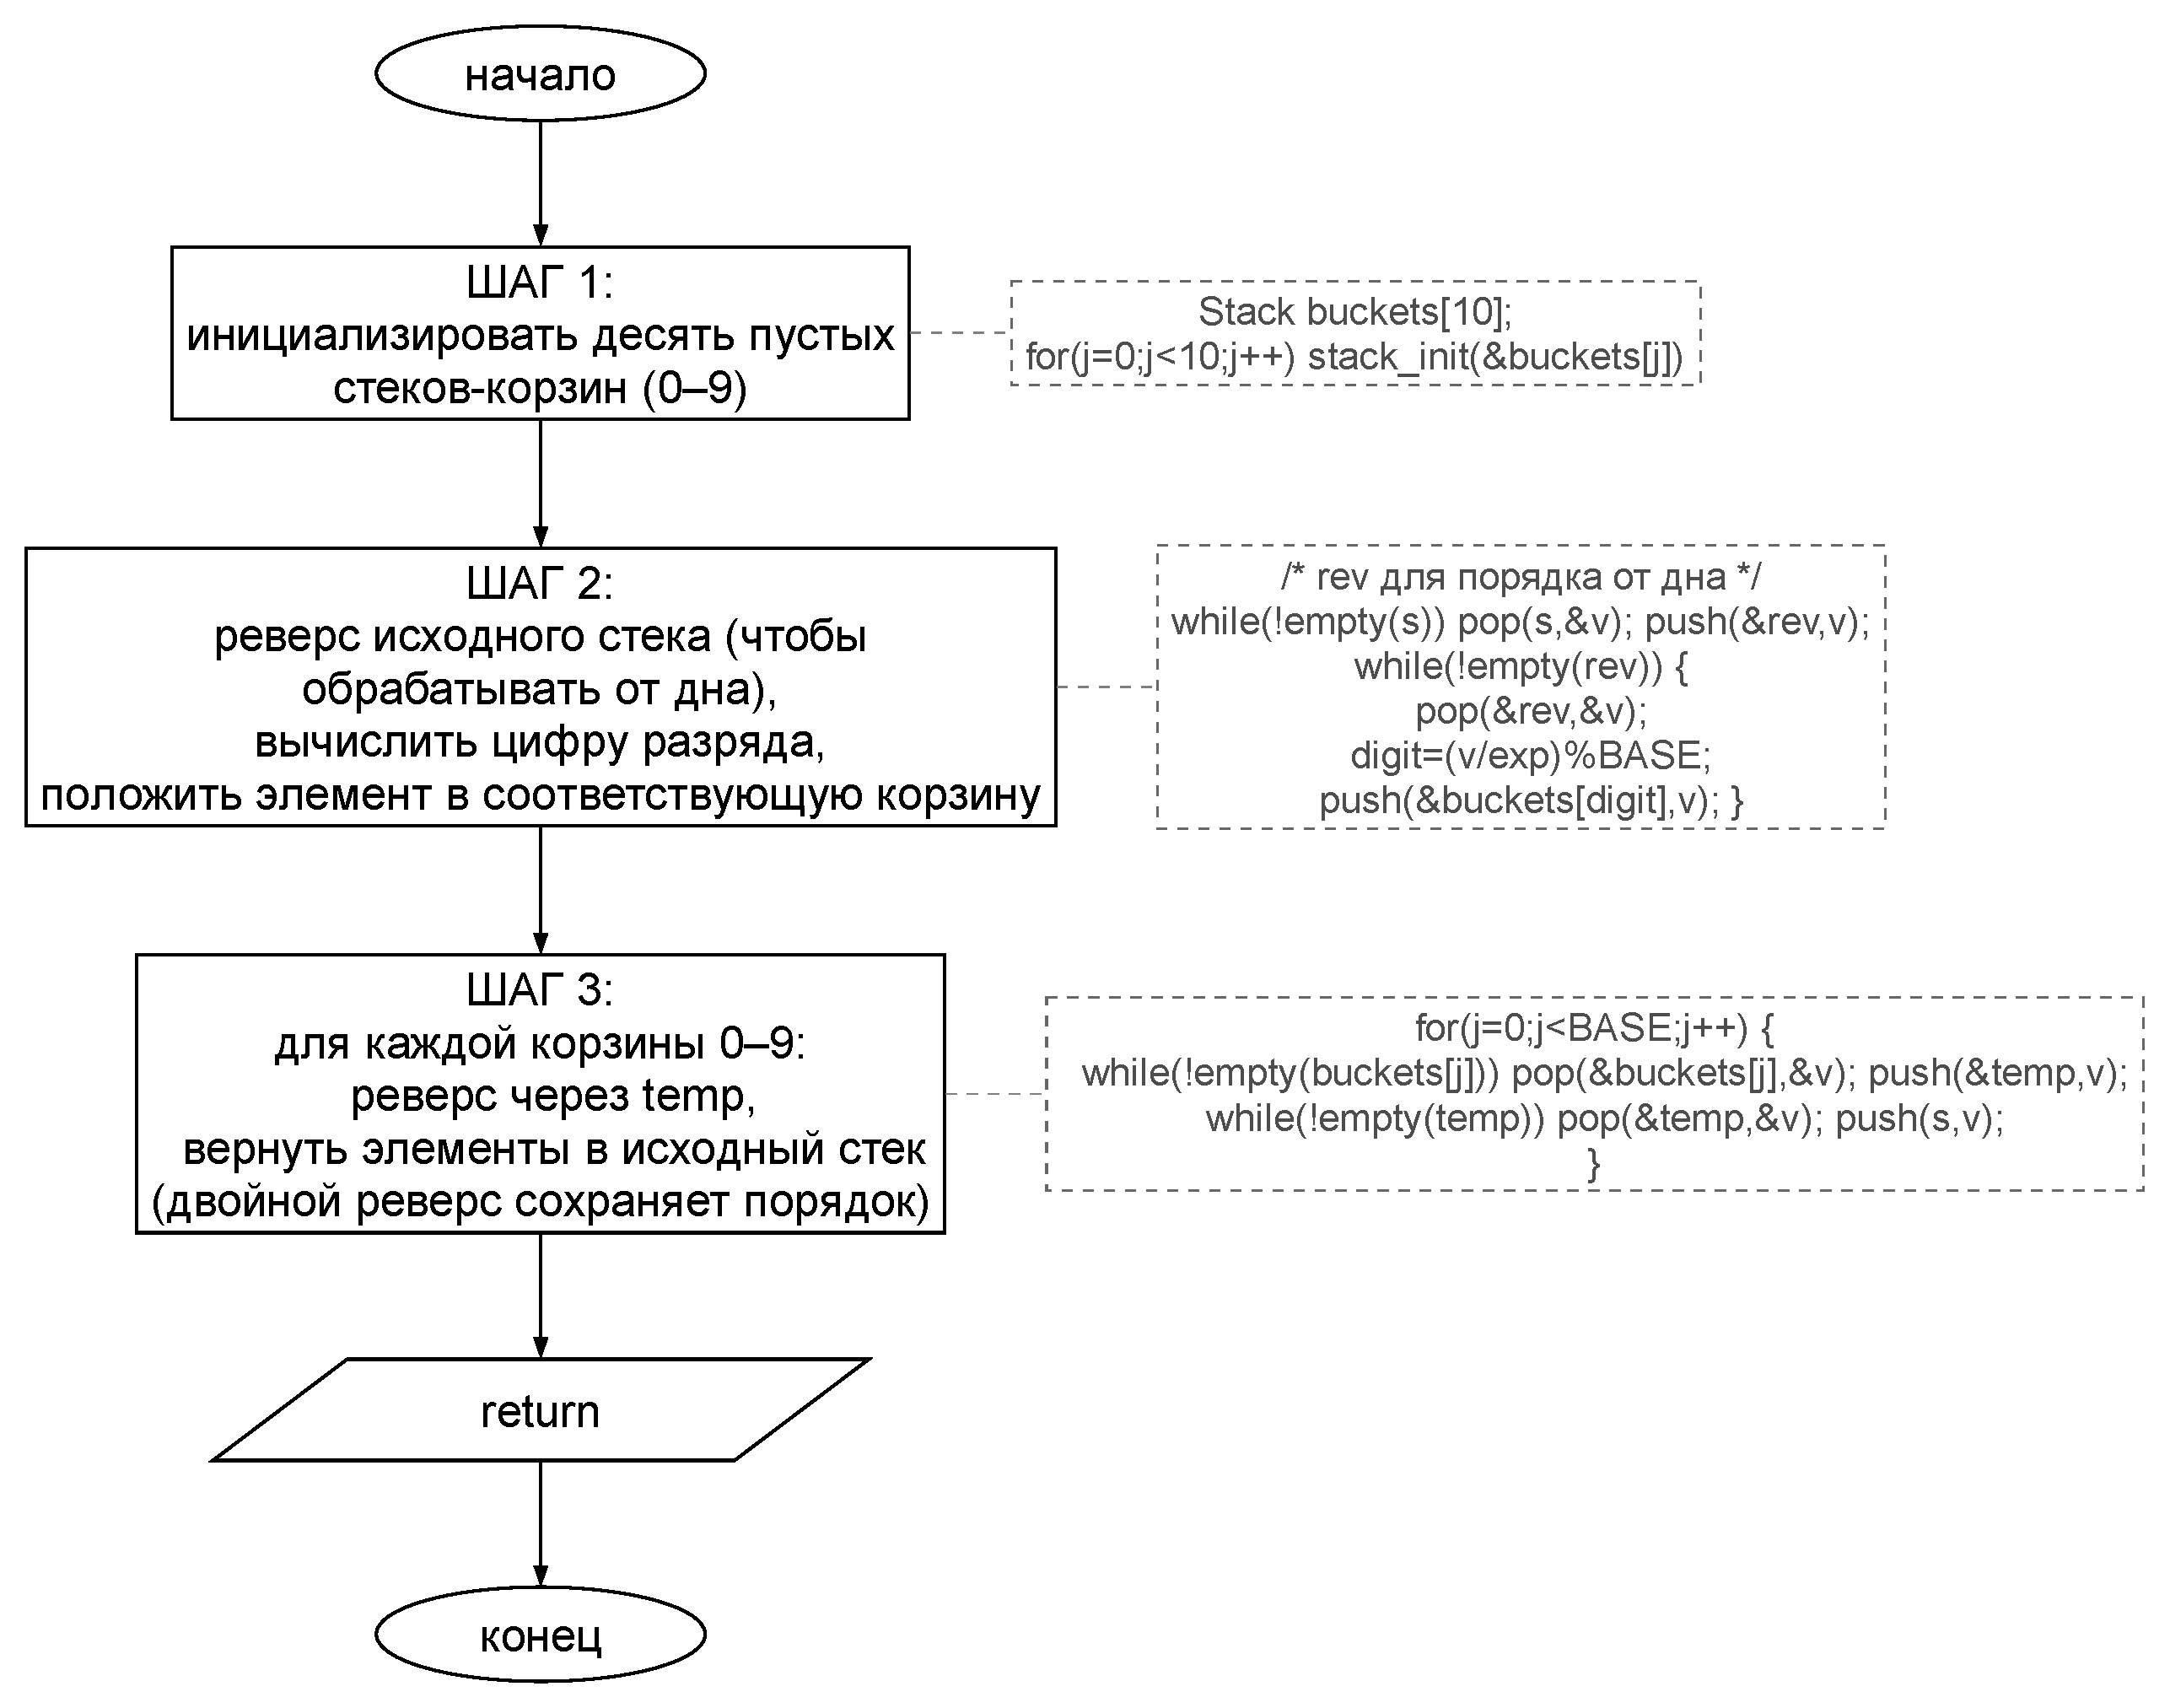
\includegraphics[width=\linewidth]{flowcharts/4_counting_sort_stack.pdf}
\caption{Блок-схема одного прохода counting\_sort\_by\_stack}
\end{figure}

\begin{landscape}
\begin{figure}[H]
\centering
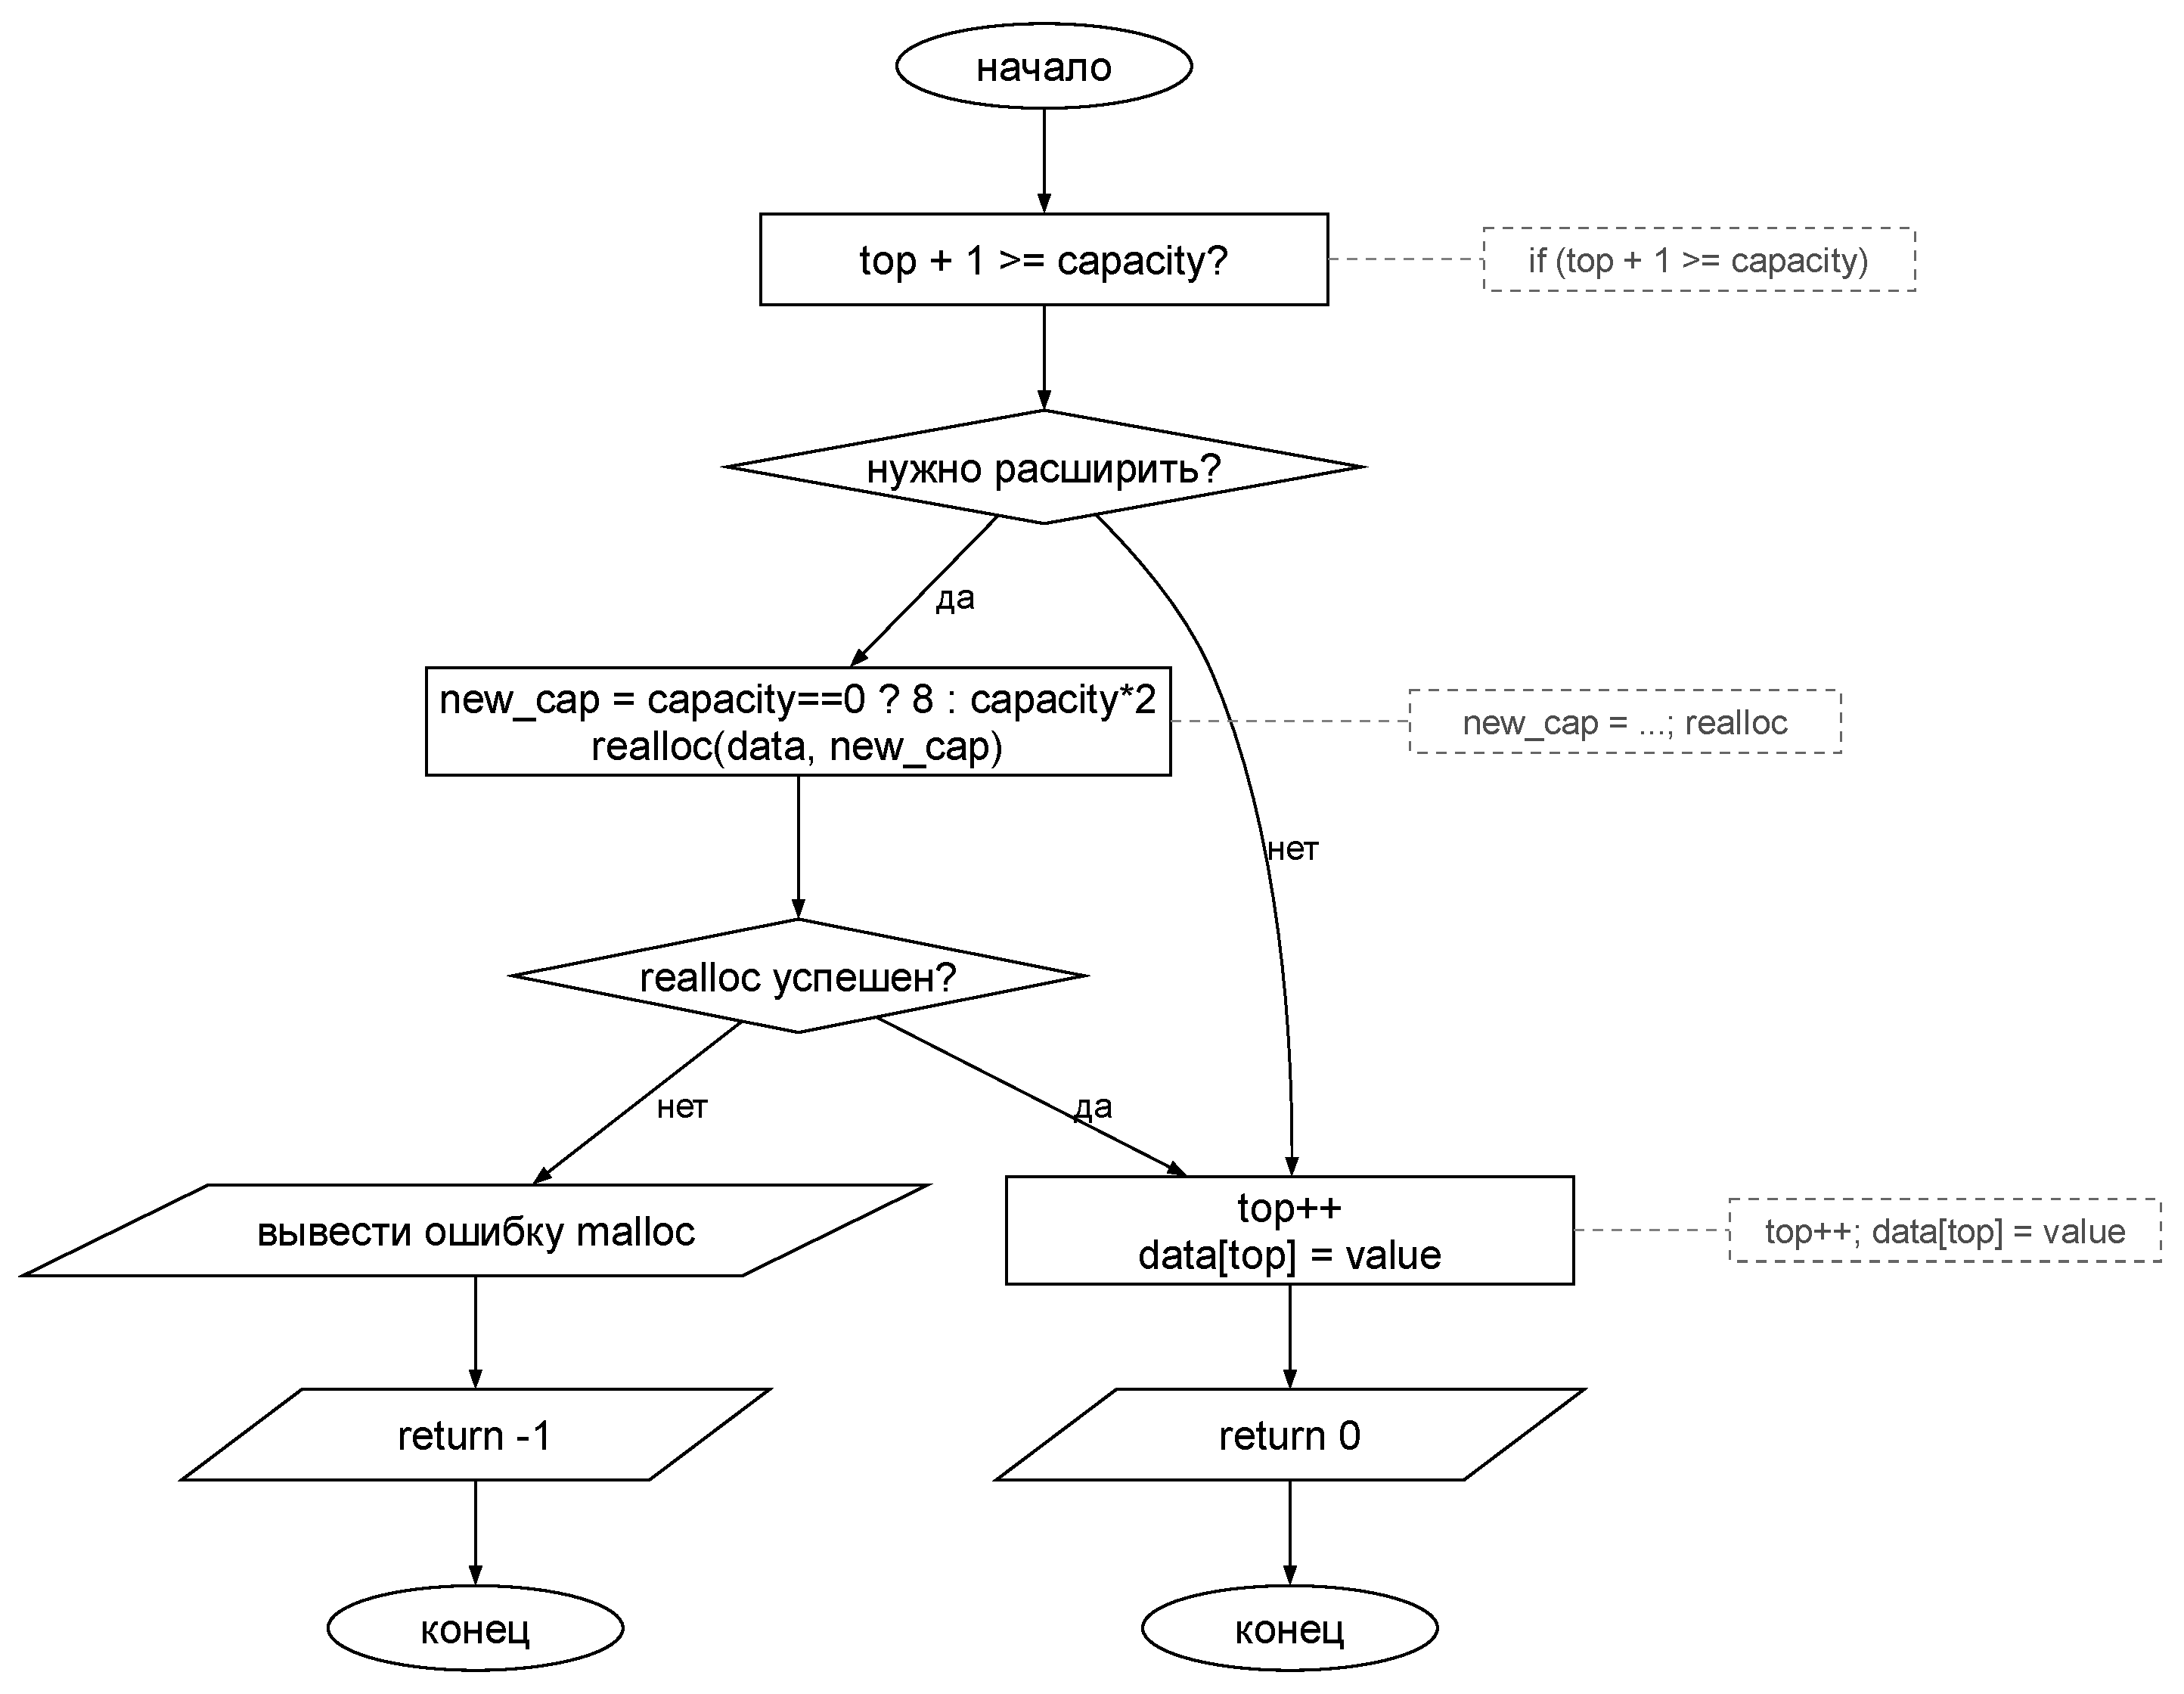
\includegraphics[width=250mm,height=155mm,keepaspectratio]{flowcharts/5a_push.pdf}
\caption{Блок-схема stack\_push}
\end{figure}
\end{landscape}

\begin{landscape}
\begin{figure}[H]
\centering
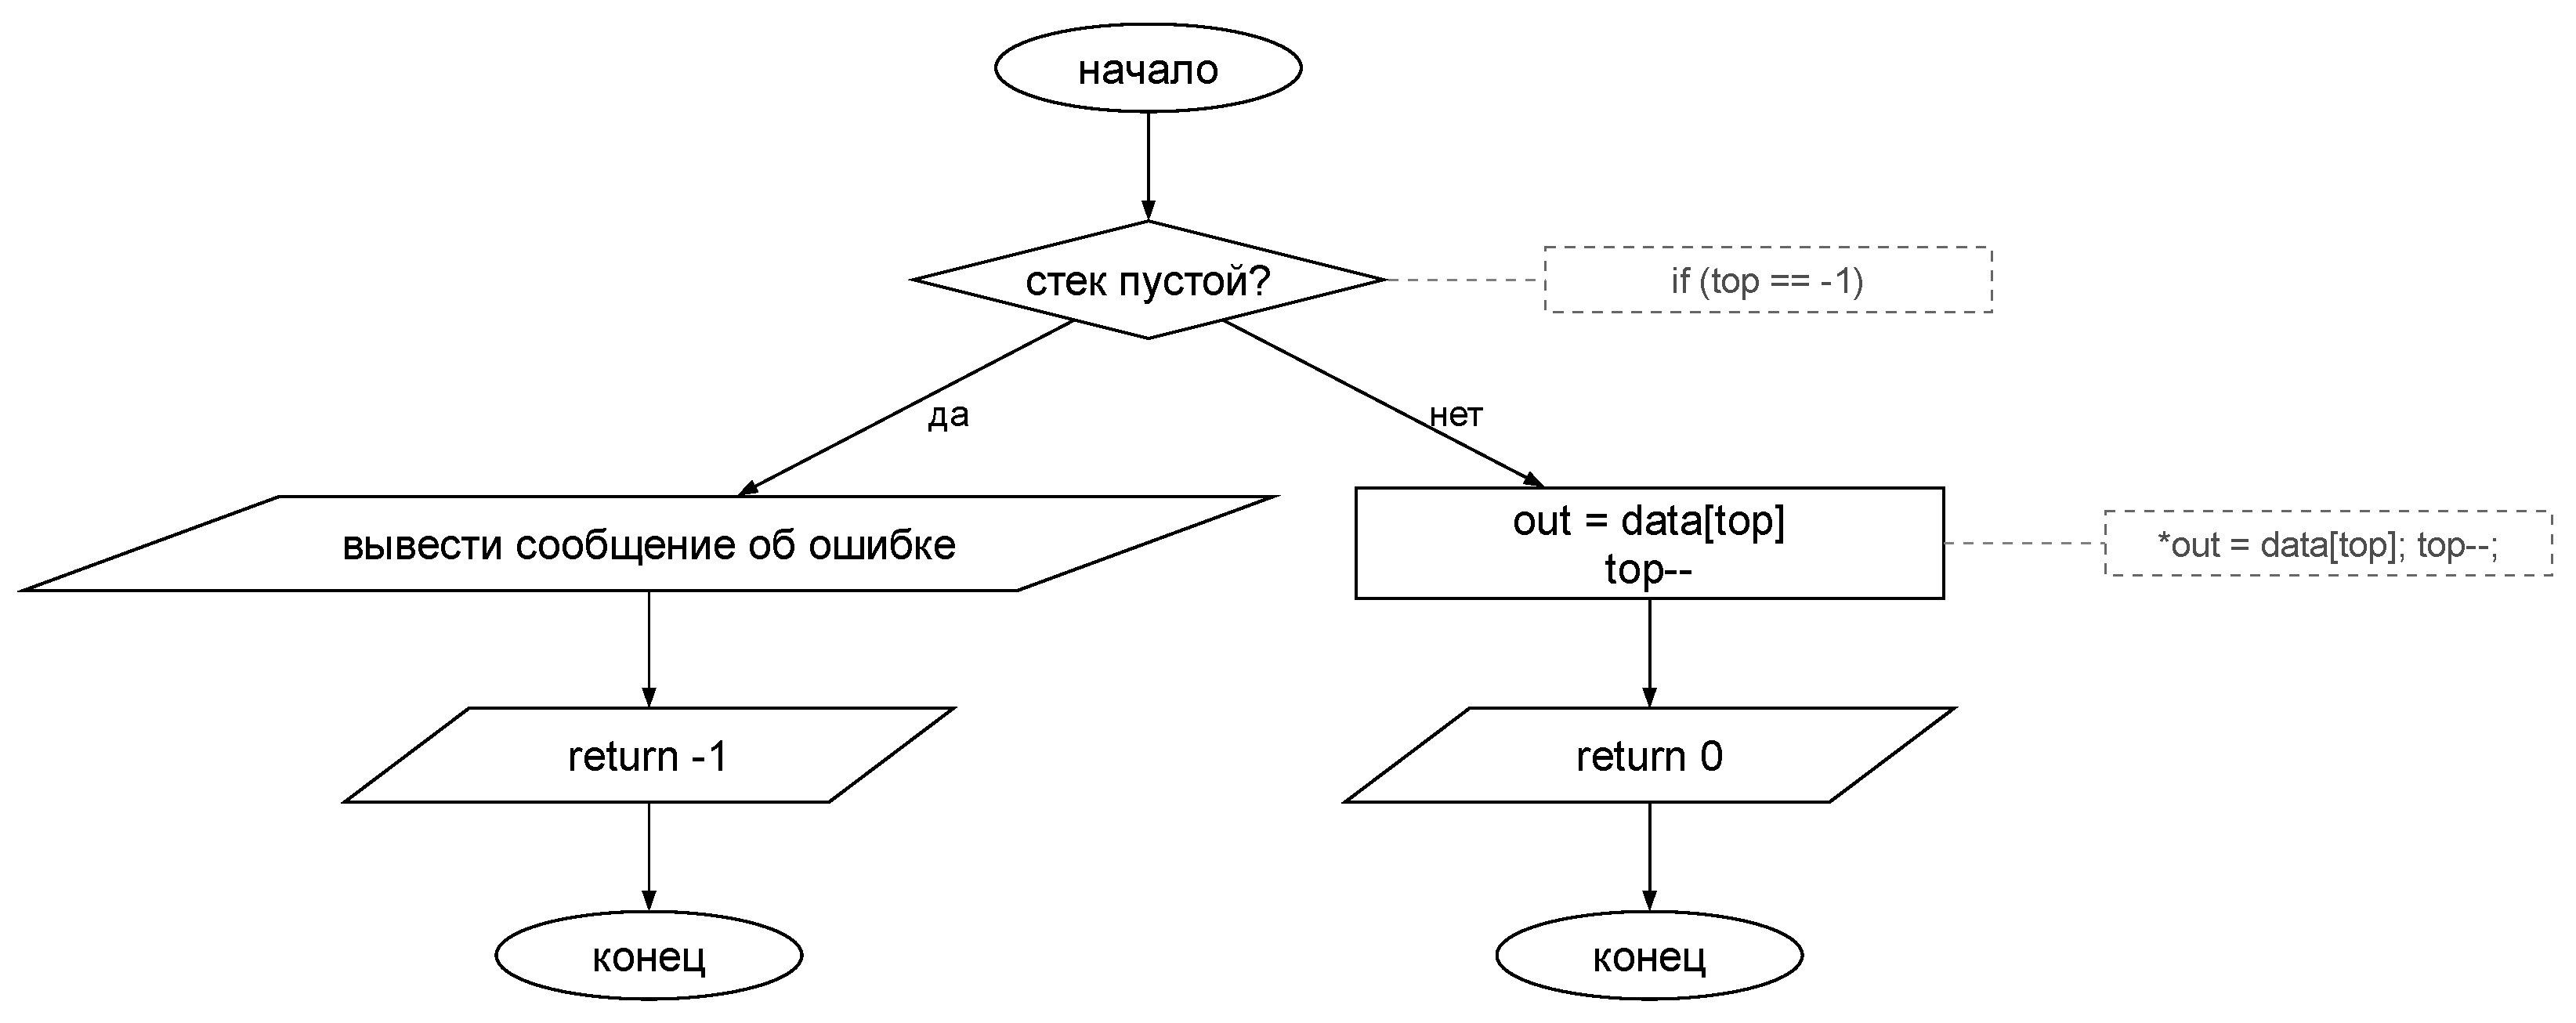
\includegraphics[width=250mm,height=155mm,keepaspectratio]{flowcharts/5b_pop.pdf}
\caption{Блок-схема stack\_pop}
\end{figure}
\end{landscape}

\begin{landscape}
\begin{figure}[H]
\centering
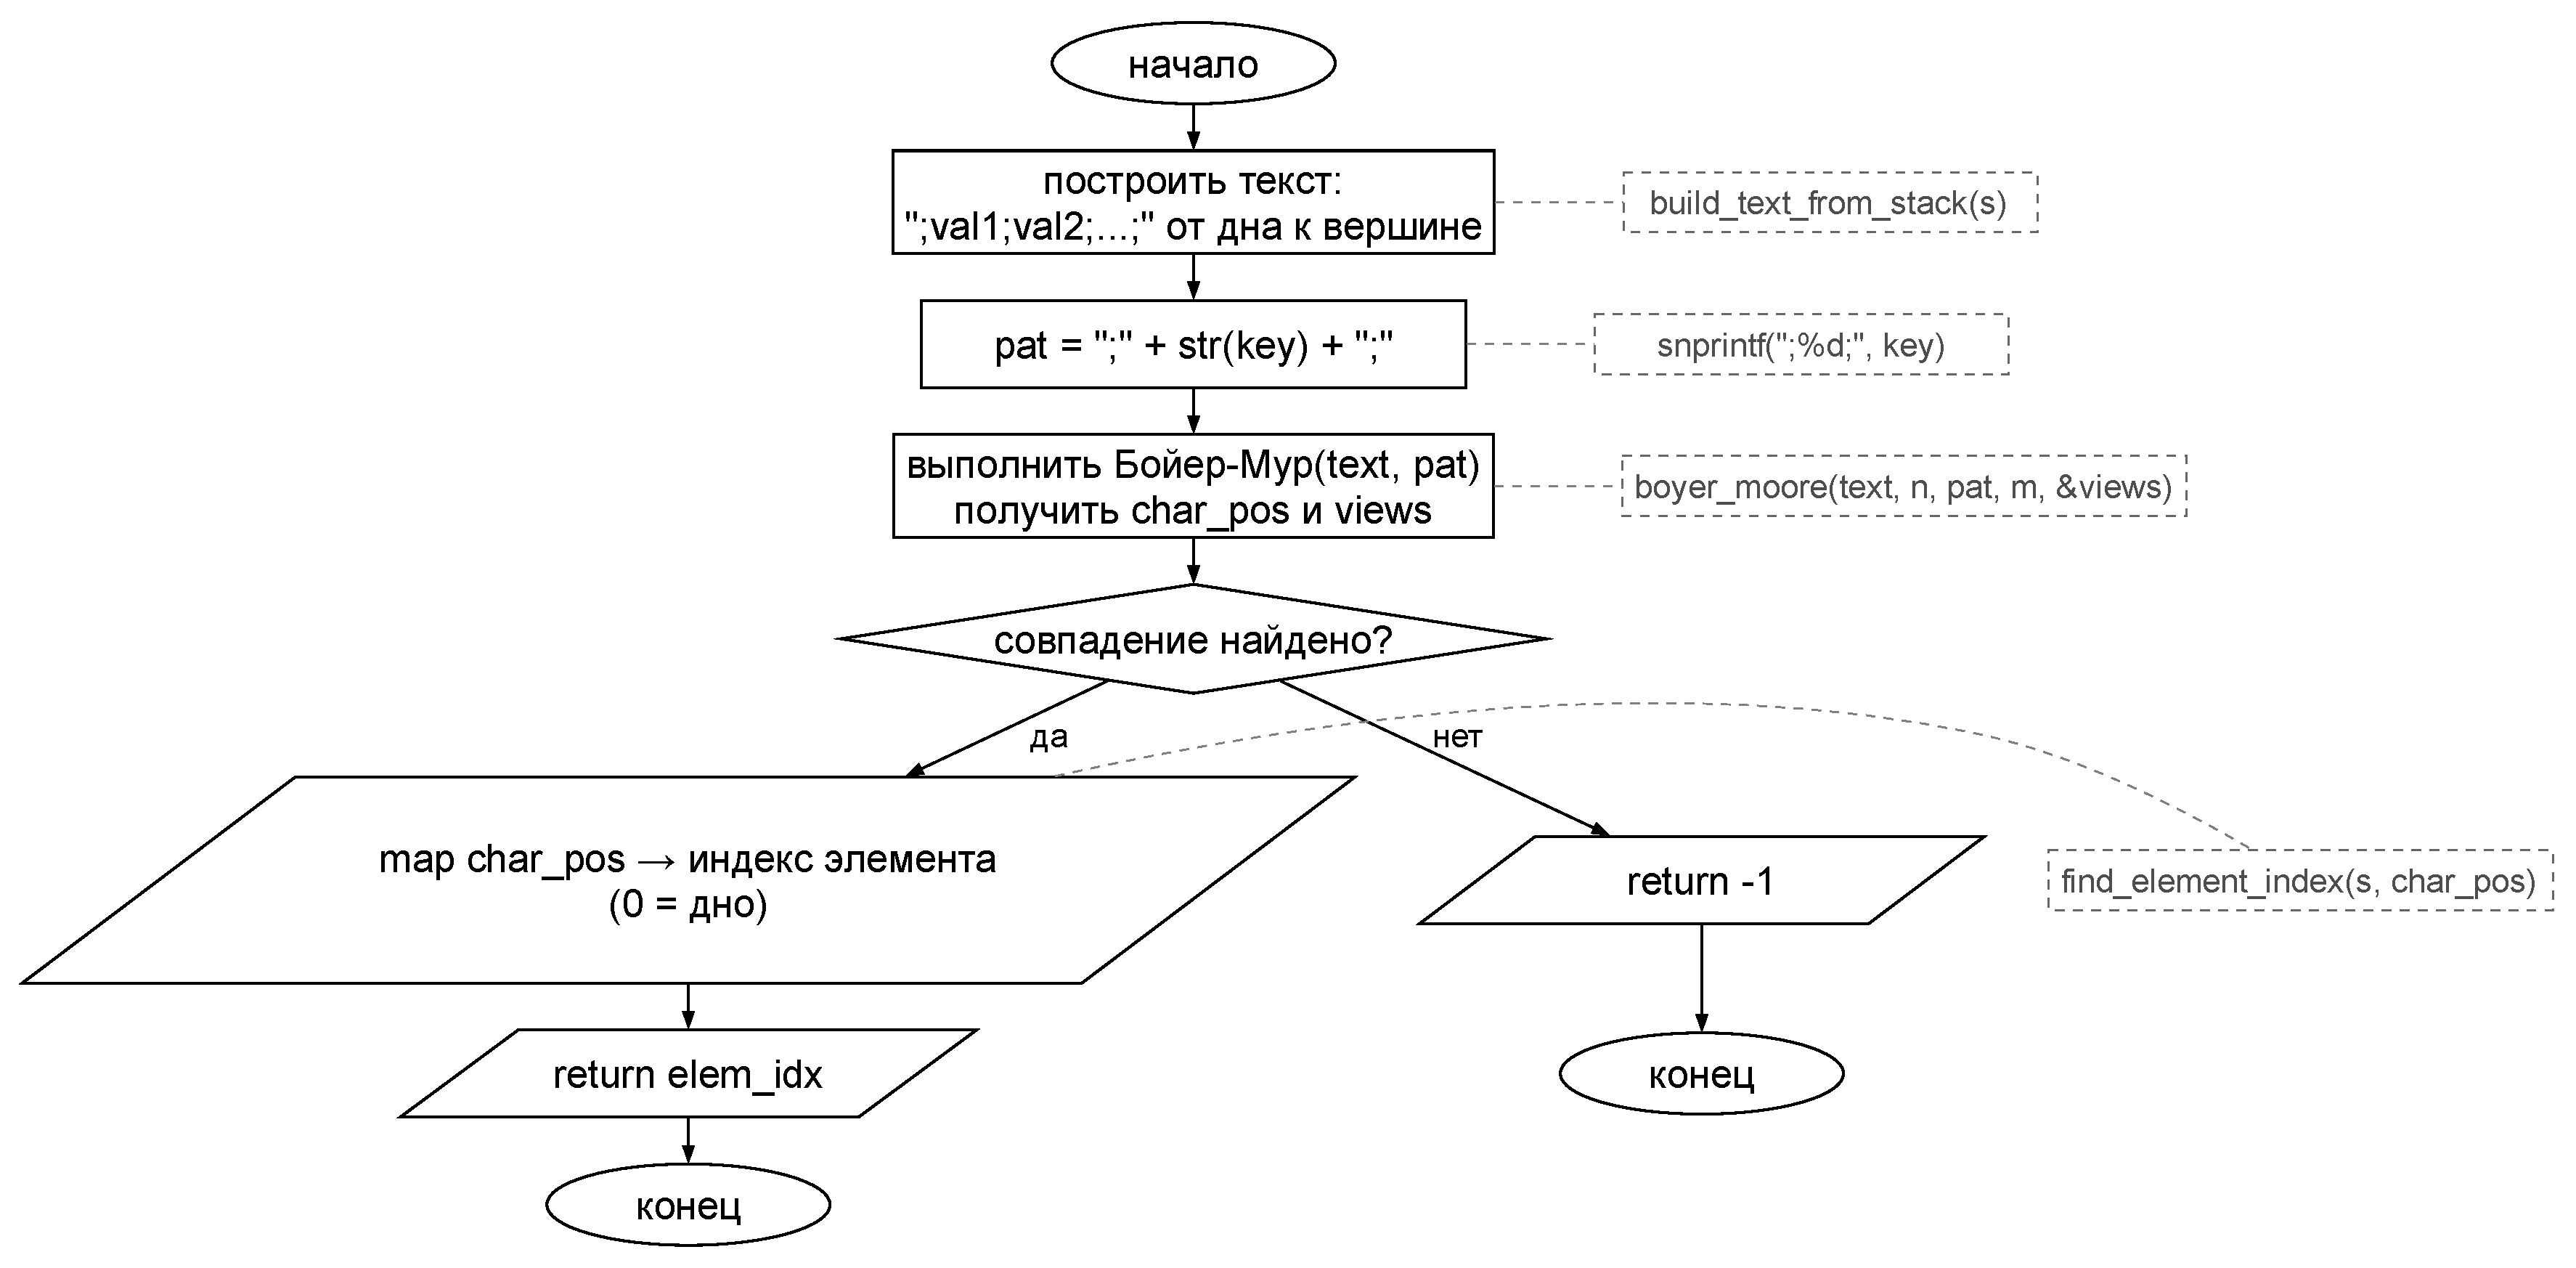
\includegraphics[width=250mm,height=155mm,keepaspectratio]{flowcharts/6_boyer_moore_search.pdf}
\caption{Блок-схема boyer\_moore\_search}
\end{figure}
\end{landscape}

\end{document}
